\documentclass[10pt,letterpaper]{article}

\usepackage[T1]{fontenc}
\usepackage{lmodern}
\usepackage[margin=0.9in]{geometry}
\usepackage{amsmath,amssymb}
\usepackage{graphicx}
\usepackage{booktabs,longtable,array}
\usepackage{xcolor}
\usepackage{listings}
\usepackage{textcomp}
\usepackage{needspace}
\usepackage{etoolbox}
\usepackage{microtype}
\usepackage{enumitem}
\usepackage{fancyhdr}
\usepackage{placeins}
\usepackage[hidelinks]{hyperref}

\definecolor{pulsusblue}{HTML}{174D73}
\definecolor{codebackground}{HTML}{F5F7F9}
\lstdefinestyle{base}{
  basicstyle=\ttfamily\small,
  backgroundcolor=\color{codebackground},
  frame=single,rulecolor=\color{black!15},
  columns=fullflexible,keepspaces=true,
  showstringspaces=false,upquote=true,breaklines=true,
  breakatwhitespace=false,tabsize=4,
  aboveskip=0.8em,belowskip=0.8em,
  xleftmargin=0.4em,xrightmargin=0.4em,
  framexleftmargin=0.35em,framexrightmargin=0.35em,
  captionpos=b
}
\lstdefinestyle{python}{style=base,language=Python,
  keywordstyle=\color{pulsusblue}\bfseries,
  commentstyle=\color{black!55},stringstyle=\color{teal!65!black}}
\lstdefinestyle{shell}{style=base,language={}}
\setlist{itemsep=0.15em,topsep=0.3em}
\setlength{\parindent}{0pt}
\setlength{\parskip}{0.3em}
\setlength{\emergencystretch}{2em}
\setlength{\headheight}{14pt}
\pagestyle{fancy}
\fancyhf{}
\fancyhead[L]{\small PULSUS User Manual}
\fancyhead[R]{\small Software 0.2.0}
\fancyfoot[C]{\thepage}
\renewcommand{\headrulewidth}{0.3pt}
\pretocmd{\section}{\Needspace{12\baselineskip}}{}{}
\pretocmd{\subsection}{\Needspace{7\baselineskip}}{}{}
\hypersetup{pdftitle={PULSUS User Manual},
  pdfauthor={Alfonso Castillo-Gonzalez},
  pdfsubject={Installation, tutorials and API reference for PULSUS 0.2.0}}

\begin{document}
\hypersetup{pageanchor=false}
\begin{titlepage}
\thispagestyle{empty}
\vspace*{1.0in}
{\color{pulsusblue}\Huge\bfseries PULSUS\par}
\vspace{0.2in}
{\LARGE User Manual\par}
\vspace{0.3in}
{\large Pulse-dressed Liouvillian Spectroscopy Using Superoperators\par}
\vspace{0.7in}
{\large Alfonso Castillo-Gonzalez\par}
\vspace{0.15in}
Manual version 0.3\quad\textbullet\quad Software version 0.2.0\par
October 15, 2026\par
\vfill
\end{titlepage}

\pagenumbering{roman}
\hypersetup{pageanchor=true}
\tableofcontents
\clearpage
\pagenumbering{arabic}
\section{Installation}
\label{sec:installation}

PULSUS requires Python~3.10 or newer. Install the released package with:
\begin{lstlisting}[style=shell]
pip install pulsus-spec
\end{lstlisting}
Then import it in Python:
\begin{lstlisting}[style=python]
import pulsus
\end{lstlisting}
The package name is \texttt{pulsus-spec}; the Python import name is
\texttt{pulsus}. NumPy, SciPy, Matplotlib and QuTiP are installed as
dependencies. The first example works in a Python script or a notebook, without
cloning the GitHub repository.

This manual describes PULSUS~0.3.0, which adds
\texttt{plot\_linear\_spectrum} and the plotters' optional
\texttt{savepath} and \texttt{dpi} arguments. These features require
version~0.3.0 or newer; if an older version is installed, upgrade with
\texttt{pip install --upgrade pulsus-spec}. The first two-dimensional
example also works with version~0.2.0.

\FloatBarrier
\section{Your first spectrum}
\label{sec:quickstart}

Two objects and two functions define the basic workflow: \texttt{SpectroscopySystem}
constructs the system, \texttt{GaussianPulse} defines a pulse,
\texttt{finite\_pulse\_spectrum} calculates the two-dimensional response,
and \texttt{plot\_spectrum} displays it.

\subsection{Copy and run the example}

The following two blocks form one complete program. Copy them, in order,
into a Python script or notebook. Only the installed package and its
standard dependencies are needed; no GitHub checkout or repository helper
is required. The example displays a figure and does not write any files.
For a script named \texttt{first\_spectrum.py}, run
\texttt{python first\_spectrum.py} from the folder containing that script.

\par\noindent
\begin{minipage}{\linewidth}
\lstinputlisting[style=python,firstline=1,lastline=36,caption={Part 1: construct the system and obtain its stationary state.},label={lst:first-spectrum}]{../../examples/manual/01_first_spectrum.py}
\end{minipage}\par

The two operators \texttt{a} and \texttt{b} lower the two-level sites.
Their energies are $1.0$ and $1.2$, with coupling $0.1$. The complete dipole
is the sum of its raising and lowering components; supplying these
components also allows the same system to be used with models that apply
the rotating-wave approximation (RWA).
Collapse operators contain square roots of the relaxation and excitation
rates. \texttt{stationary\_state()} returns a density matrix; pass that
matrix explicitly as \texttt{rho0} in the calculation.

\par\noindent
\begin{minipage}{\linewidth}
\lstinputlisting[style=python,firstline=38,lastline=66,caption={Part 2: calculate and display the spectrum.}]{../../examples/manual/01_first_spectrum.py}
\end{minipage}\par

The same pulse is used for all three interactions. Its \texttt{sigma}
is the standard deviation of the Gaussian field envelope. With
$\hbar=1$, frequencies and rates are in inverse model time units;
\texttt{sigma} and the waiting time \texttt{T} use model time units.
\texttt{pathway="NR"} selects the nonrephasing convention.
Positive \texttt{eta} ensures causal-transform convergence and adds
broadening; Section~\ref{sec:linear} explains its choice.

The result is a complex array with shape
$(\mathrm{len}(\omega_3),\mathrm{len}(\omega_1))$:
\texttt{S[j, i]} corresponds to \texttt{omega3[j]} and
\texttt{omega1[i]}. Here the shape is $(31,31)$.
\texttt{component="imag"} selects the imaginary part for display;
\texttt{normalize=True} divides that displayed component by its maximum
absolute value. The complex array \texttt{S} remains available for further
calculations.

\begin{figure}[!htbp]
\centering
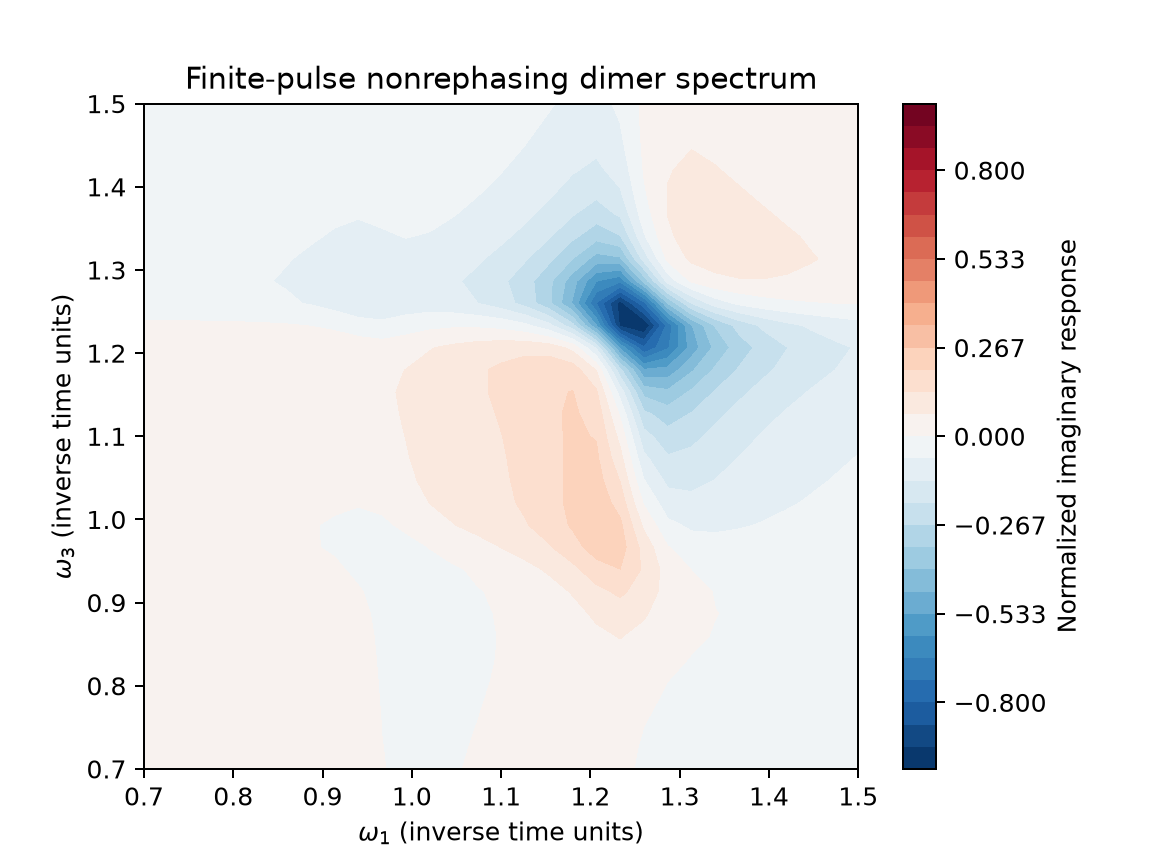
\includegraphics[width=0.78\linewidth]{figures/first_nr_spectrum.png}
\caption{Output of the first example: normalized imaginary nonrephasing
response on a $31\times31$ frequency grid. The horizontal coordinate is
$\omega_1$ and the vertical coordinate is $\omega_3$, both in inverse model
time units. The color scale shows the signed imaginary response.}
\label{fig:first-spectrum}
\end{figure}

\subsection{Choose a model}
\label{sec:models-at-a-glance}

Five functions calculate third-order spectra on the same type of
frequency grid. The RWA retains resonant raising and lowering interactions. The first four models form
an approximation ladder; the full impulsive function is an additional
molecular reference.

\begin{longtable}{@{}p{0.49\linewidth}p{0.45\linewidth}@{}}
\toprule
\textbf{Function} & \textbf{Calculation} \\
\midrule
\endhead
\texttt{finite\_pulse\_spectrum} (A) &
Full interaction with finite Gaussian pulse dressing. \\
\texttt{finite\_pulse\_rwa\_spectrum} (B) &
Finite Gaussian pulse dressing with RWA interactions. \\
\texttt{short\_pulse\_rwa\_spectrum} (C) &
RWA molecular response multiplied by scalar Gaussian spectral envelopes. \\
\texttt{impulsive\_rwa\_spectrum} (D) &
RWA molecular response without pulse filtering or field prefactors. \\
\texttt{impulsive\_spectrum} &
Full-interaction molecular response without pulses or an R/NR selector. \\
\bottomrule
\end{longtable}

To use B or C in the first example, replace the spectrum function with
one of the following, keeping the same arguments:
\begin{itemize}
\item \texttt{pulsus.finite\_pulse\_rwa\_spectrum}
\item \texttt{pulsus.short\_pulse\_rwa\_spectrum}
\end{itemize}
The example already supplies the dipole components required by the RWA.
For D, omit the three pulse arguments:
\begin{lstlisting}[style=python]
S = pulsus.impulsive_rwa_spectrum(
    system=system,
    omega1=omega1, omega3=omega3,
    T=20.0, eta=0.02,
    pathway="NR", rho0=rho_ss,
)
\end{lstlisting}
For the full impulsive model, use \texttt{pulsus.impulsive\_spectrum}
and also omit \texttt{pathway}. Impulsive functions return a molecular
response without the Gaussian field factors, so their absolute amplitudes
are not on the same scale as the finite-pulse calculation.

For a one-dimensional spectrum, use a linear spectrum function.
Section~\ref{sec:linear} introduces the four linear models and their
calling patterns. Section~\ref{sec:third-order} develops
the third-order models and R/NR conventions in more detail.

\FloatBarrier
\section{Scientific scope}
\label{sec:introduction}

PULSUS calculates linear and third-order response functions for open
quantum systems. It evaluates frequency-domain spectra directly from the
field-free Liouvillian, so a time-domain interferogram is not needed first.

\subsection{Supported systems}
Provide the Hamiltonian, dipole and collapse operators as finite matrices.
The package supports coupled electronic models and other systems that can
be represented in a finite basis. For a Hilbert-space dimension $d$, each
operator is $d\times d$ and the dense Liouvillian is $d^2\times d^2$.
The matrix size therefore sets the computational cost; selected-coordinate
calculations reduce the number of spectral points evaluated.

\subsection{Assumptions of the finite-pulse calculation}
The standard finite-pulse formulation uses a time-independent Markovian
Lindblad generator, electric-dipole coupling, Gaussian pulses with ordered,
separated interactions, and a stationary initial state under the field-free
Liouvillian. Use \texttt{system.stationary\_state()} to obtain that state and
pass it explicitly as \texttt{rho0}. Although several functions accept
other density matrices, accepting a matrix does not establish the validity
of the standard finite-pulse formula for a nonstationary preparation.

The public time-domain functions implement impulsive interactions.
Finite-duration driven time propagation, non-Markovian dynamics,
time-dependent field-free generators, and automatic construction of
molecular Hamiltonians or dipole components are outside the documented
production interface.

\subsection{Calculation workflow}
\begin{enumerate}
\item Construct the system in a consistent unit system and prepare its state.
\item Define Gaussian pulses for a finite-pulse or short-pulse model.
\item Select a response model, R/NR convention, waiting time and frequency axes.
\item Calculate the complex response and display the desired component.
\end{enumerate}

\FloatBarrier
\section{Defining systems, initial states, and pulses}
\label{sec:systems}

\subsection{The system object}

\texttt{SpectroscopySystem} groups the Hamiltonian, detection dipole,
Lindblad collapse operators, and optional initial state. Its constructor is
\par\noindent
\begin{minipage}{\linewidth}
\begin{lstlisting}[style=python]
system = pulsus.SpectroscopySystem(
    H, dipole, collapse_ops=None, rho0=None, hbar=1.0,
    dipole_plus=None, dipole_minus=None,
)
\end{lstlisting}
\end{minipage}\par
The first two arguments are required. For Hilbert-space dimension $d$,
\texttt{H} and \texttt{dipole} must be dense $d\times d$ matrices. Supply the
same dimensions for each collapse operator, the initial density matrix, and
the two optional dipole components. NumPy arrays and nested Python lists
are suitable inputs; SciPy sparse matrices are not a supported input format
in this release. The implementation converts matrices to complex NumPy
arrays and constructs dense superoperators of size $d^2\times d^2$.

The field-free equation of motion is
\begin{equation}
 \dot\rho=-\frac{i}{\hbar}[H,\rho]
 +\sum_k\left(C_k\rho C_k^\dagger
 -\frac{1}{2}\{C_k^\dagger C_k,\rho\}\right).
\end{equation}
The interaction superoperator uses
$\mathcal V\rho=(i/\hbar)[\mu,\rho]$. The sign and Fourier conventions are
therefore already built into PULSUS; do not insert additional factors of
$i$ into a spectrum simply to match an assumed plotting convention.

The object exposes \texttt{H}, \texttt{dipole}, \texttt{collapse\_ops},
\texttt{rho0}, \texttt{hbar}, and \texttt{d}. Its precomputed
\texttt{L} and \texttt{V} are the field-free and full interaction
superoperators. When dipole components are supplied, \texttt{V\_plus} and
\texttt{V\_minus} are constructed as well. Rebuild the object when changing
the Hamiltonian, dipole, dissipation, or $\hbar$: editing an attribute does
not automatically recompute the corresponding superoperators.

\subsection{Collapse operators contain their rates}

For a decay channel with rate $\gamma$ and lowering operator $a$, supply
$C=\sqrt{\gamma}\,a$, rather than $\gamma a$. The dissipator is quadratic in
$C$. The dimer tutorial also includes excitation with occupation parameter
$\bar n$:
\par\noindent
\begin{minipage}{\linewidth}
\begin{lstlisting}[style=python]
gamma = 0.05
nbar = 0.05
collapse_ops = [
    np.sqrt(gamma * (nbar + 1.0)) * a,
    np.sqrt(gamma * nbar) * a.conj().T,
    np.sqrt(gamma * (nbar + 1.0)) * b,
    np.sqrt(gamma * nbar) * b.conj().T,
]
\end{lstlisting}
\end{minipage}\par
Here $a$ and $b$ act on their respective sites in the full tensor-product
space. A single-site $2\times2$ collapse operator cannot be inserted into
the four-state dimer without the tensor-product extension. These local
excitation and decay terms define the model's bath; their stationary state
should not be assumed to equal a Gibbs state of an arbitrary coupled
Hamiltonian.

\subsection{Choose one consistent unit system}

PULSUS does not convert units. All arguments must be consistent with the
equations above. In the tutorial, $\hbar=1$: Hamiltonian entries,
\texttt{omega\_L}, \texttt{omega1}, \texttt{omega3}, \texttt{eta}, and
decay rates use inverse model-time units; \texttt{sigma}, \texttt{T}, and
time axes use the corresponding model-time unit. Frequencies are angular
frequencies, not cycles per unit time.

For energies in eV and times in fs, one consistent choice is
\par\noindent
\begin{minipage}{\linewidth}
\begin{lstlisting}[style=python]
hbar_eV_fs = 0.6582119569
system = pulsus.SpectroscopySystem(
    H=H_eV,
    dipole=dipole,
    collapse_ops=collapse_ops_per_sqrt_fs,
    hbar=hbar_eV_fs,
)
omega_L = photon_energy_eV / hbar_eV_fs
omega_axis = energy_axis_eV / hbar_eV_fs
\end{lstlisting}
\end{minipage}\par
In this convention, \texttt{sigma} and \texttt{T} are in fs and
\texttt{eta} and $\gamma$ are in fs$^{-1}$. A population lifetime
$\tau$ gives $\gamma=1/\tau$ in the chosen time unit. Include
$\sqrt\gamma$ in each collapse operator once. The code divides Hamiltonian
and interaction commutators by $\hbar$; it does not divide the Lindblad
dissipator by $\hbar$. Do not apply an extra $1/\hbar$ to rates that already
have inverse-time units. The product of dipole and field amplitude must
also have energy units if absolute physical polarization amplitudes are
required. The illustrative examples use model dipoles and fields.

\subsection{The state before the first pulse}

\texttt{rho0} is the system's density matrix immediately before the first
interaction. Its diagonal entries give populations; its off-diagonal
entries describe coherences. For a $d$-state model, supply a complex
$d\times d$ matrix with trace one.

The tutorials start from a stationary state: a state that does not change
under the Hamiltonian and dissipation before the pulses arrive. Calculate
that state once, then pass it to the spectrum calculation:
\par\noindent
\begin{minipage}{\linewidth}
\begin{lstlisting}[style=python]
rho_ss = system.stationary_state()
S = pulsus.finite_pulse_spectrum(
    system=system,
    pulse1=pulse, pulse2=pulse, pulse3=pulse,
    omega1=omega1, omega3=omega3, T=20.0, eta=0.02,
    pathway="NR", rho0=rho_ss,
)
\end{lstlisting}
\end{minipage}\par

The method returns the matrix; it does not assign
\texttt{system.rho0}. An explicit \texttt{rho0} in a function call takes
priority over a state stored in the system. If neither is supplied,
PULSUS raises an error rather than choosing a state for you.

The standard finite-pulse formulation assumes stationary preparation.
For a model with several possible stationary states, choose the state
that matches the intended preparation. The solver returns one stationary
candidate and does not determine whether it is unique.

\subsection{Dipole components for the rotating-wave approximation}

Full-interaction calculations require only \texttt{dipole}. RWA
calculations additionally require both \texttt{dipole\_plus} and
\texttt{dipole\_minus}. PULSUS does not infer them from \texttt{H}.
For the excitation-conserving dimer in the first tutorial,
\par\noindent
\begin{minipage}{\linewidth}
\begin{lstlisting}[style=python]
dipole_plus = a.conj().T + b.conj().T
dipole_minus = dipole_plus.conj().T
dipole = dipole_plus + dipole_minus
system = pulsus.SpectroscopySystem(
    H=H, dipole=dipole, collapse_ops=collapse_ops,
    hbar=1.0, dipole_plus=dipole_plus,
    dipole_minus=dipole_minus,
)
rho_ss = system.stationary_state()
\end{lstlisting}
\end{minipage}\par
The raising/lowering definition must match the physical transition
structure of the user's model. A matrix that happens to be triangular in
an arbitrary basis is not automatically its positive-frequency dipole.
The RWA functions use \texttt{V\_plus} for field sign $+1$ and
\texttt{V\_minus} for sign $-1$; detection still uses the full dipole.

\subsection{GaussianPulse and pulse duration}

\par\noindent
\begin{minipage}{\linewidth}
\begin{lstlisting}[style=python]
pulse = pulsus.GaussianPulse(
    omega_L=1.10, sigma=1.25, E0=1.0, phase=0.0,
)
\end{lstlisting}
\end{minipage}\par

\texttt{omega\_L} is the carrier angular frequency and \texttt{sigma}
is the temporal width of the field envelope. Both are required.
\texttt{E0} is the peak field amplitude (default 1.0), and
\texttt{phase} is in radians (default 0.0). To change pulse parameters,
create a new \texttt{GaussianPulse}.

PULSUS uses the field envelope $\exp[-t^2/(2\sigma^2)]$.
If a pulse duration is given as a full width at half maximum (FWHM),
convert it to \texttt{sigma} before creating the pulse:
\begin{equation}
 \sigma=\frac{\mathrm{FWHM}_{E}}{2\sqrt{2\ln2}}
       \simeq\frac{\mathrm{FWHM}_{E}}{2.355},
 \qquad
 \sigma=\frac{\mathrm{FWHM}_{I}}{2\sqrt{\ln2}}
       \simeq\frac{\mathrm{FWHM}_{I}}{1.665}.
\end{equation}
Here $E$ means the \emph{field-amplitude envelope} and $I$ means the
\emph{intensity envelope}, proportional to the squared field envelope.
Use the formula matching the stated duration; neither FWHM is
\texttt{sigma} itself. Larger \texttt{sigma} gives a longer pulse with a
narrower frequency bandwidth.

When changing the duration, keeping \texttt{E0} fixed keeps the peak
field fixed. The pulse area then changes with \texttt{sigma}. To compare
fixed envelope areas instead, choose $E_0\propto1/\sigma$. Finite-pulse
and short-pulse results include field-amplitude factors; impulsive
molecular responses do not. Normalizing each plot separately removes
those amplitude differences from the display.

\FloatBarrier
\section{Linear spectroscopy}
\label{sec:linear}

\subsection{Choose a linear model}

Linear spectrum functions take the system, a one-dimensional angular-frequency
axis and the convergence parameter \texttt{eta}. Pulse-dependent functions
also take a \texttt{GaussianPulse}. Each returns a complex array with one
entry per frequency.


The positive parameter \texttt{eta}, in inverse time units, ensures
convergence of the causal frequency transform. For a stable field-free
Liouvillian,
\[
G_\eta(\omega)=\int_0^\infty
 e^{(i\omega-\eta)t}e^{\mathcal L t}\,dt
 =[(\eta-i\omega)I-\mathcal L]^{-1}.
\]
The factor $e^{-\eta t}$ makes the integral decay, but also adds broadening
beyond the physical relaxation and dephasing in the collapse operators.
When using \texttt{eta} only for convergence, choose a small positive value
that does not materially change the spectral features and still permits
stable linear solves. Reduce it and refine the frequency grid together;
compare unnormalized complex responses, including widths and amplitudes.
The tutorial value $\eta=0.02$ is illustrative, not a universal optimum.

\begin{description}
\item[\texttt{finite\_pulse\_linear\_spectrum}]
Gaussian pulse dressing with the full molecular interaction.
\item[\texttt{impulsive\_linear\_spectrum}]
Full molecular interaction in the impulsive limit, without a pulse envelope.
\item[\texttt{short\_pulse\_linear\_rwa\_spectrum}]
RWA molecular response weighted by the Gaussian pulse spectrum.
\item[\texttt{impulsive\_linear\_rwa\_spectrum}]
RWA molecular response in the impulsive limit, without a pulse envelope.
\end{description}
There is no finite-pulse linear RWA function in this version. The four
available functions have these calling patterns:

\par\noindent
\begin{minipage}{\linewidth}
\begin{lstlisting}[style=python]
finite_pulse_linear_spectrum(
    system, pulse, omega, eta, sign=1, rho0=None)
impulsive_linear_spectrum(system, omega, eta, rho0=None)
short_pulse_linear_rwa_spectrum(
    system, pulse, omega, eta, sign=1, rho0=None)
impulsive_linear_rwa_spectrum(
    system, omega, eta, sign=1, rho0=None)
\end{lstlisting}
\end{minipage}\par
The RWA calls need the two dipole components supplied in the first example.
Use \texttt{sign=1} for the positive-frequency field component.

\subsection{Compare the four models}

Continue in the same Python session as the first example, where
\texttt{system} and \texttt{rho\_ss} have been defined. The code below creates
\emph{one figure with two panels}: the real part on the left and the imaginary
part on the right. Both panels contain all four models.

For this comparison the Gaussian prefactor is set to one at zero phase.
Each complex curve is then divided by its own maximum magnitude so that the
figure compares shapes. These separately normalized curves do not compare
absolute amplitudes. The plotting helper uses \texttt{normalize=False}
to retain this common scale for both components. Its optional
\texttt{normalize=True} instead scales the selected real, imaginary or
absolute-value component by that component's own maximum absolute value.

\par\noindent
\begin{minipage}{\linewidth}
\begin{lstlisting}[style=python]
omega = np.linspace(0.5, 1.7, 241)
sigma = 1.25
pulse = pulsus.GaussianPulse(
    omega_L=1.10, sigma=sigma,
    E0=2 / (np.sqrt(2 * np.pi) * sigma),
)
shared = dict(system=system, omega=omega, eta=0.02,
              rho0=rho_ss)
spectra = {
    "Finite pulse, full": pulsus.finite_pulse_linear_spectrum(
        pulse=pulse, sign=1, **shared),
    "Impulsive, full": pulsus.impulsive_linear_spectrum(**shared),
    "Short pulse, RWA": pulsus.short_pulse_linear_rwa_spectrum(
        pulse=pulse, sign=1, **shared),
    "Impulsive, RWA": pulsus.impulsive_linear_rwa_spectrum(
        sign=1, **shared),
}
fig, axes = plt.subplots(1, 2, figsize=(10, 3.8),
                         constrained_layout=True)
styles = ["-", "--", "-.", ":"]
for (name, spectrum), style in zip(spectra.items(), styles):
    scale = np.max(np.abs(spectrum))
    y = spectrum / scale if scale else spectrum
    for ax, component in zip(axes, ["real", "imag"]):
        pulsus.plot_linear_spectrum(
            omega, y, component=component, normalize=False,
            ax=ax, label=name, linestyle=style, linewidth=1.1,
        )
for ax, component in zip(axes, ["Real", "Imaginary"]):
    ax.set_xlabel("Angular frequency (inverse model time)")
    ax.set_ylabel(component + " response / max |complex response|")
    ax.set_title(component + " part: all four models")
    ax.axhline(0, color="0.7", lw=0.6)
    ax.legend(fontsize=7)
plt.show()
\end{lstlisting}
\end{minipage}\par

\begin{figure}[!htbp]
\centering
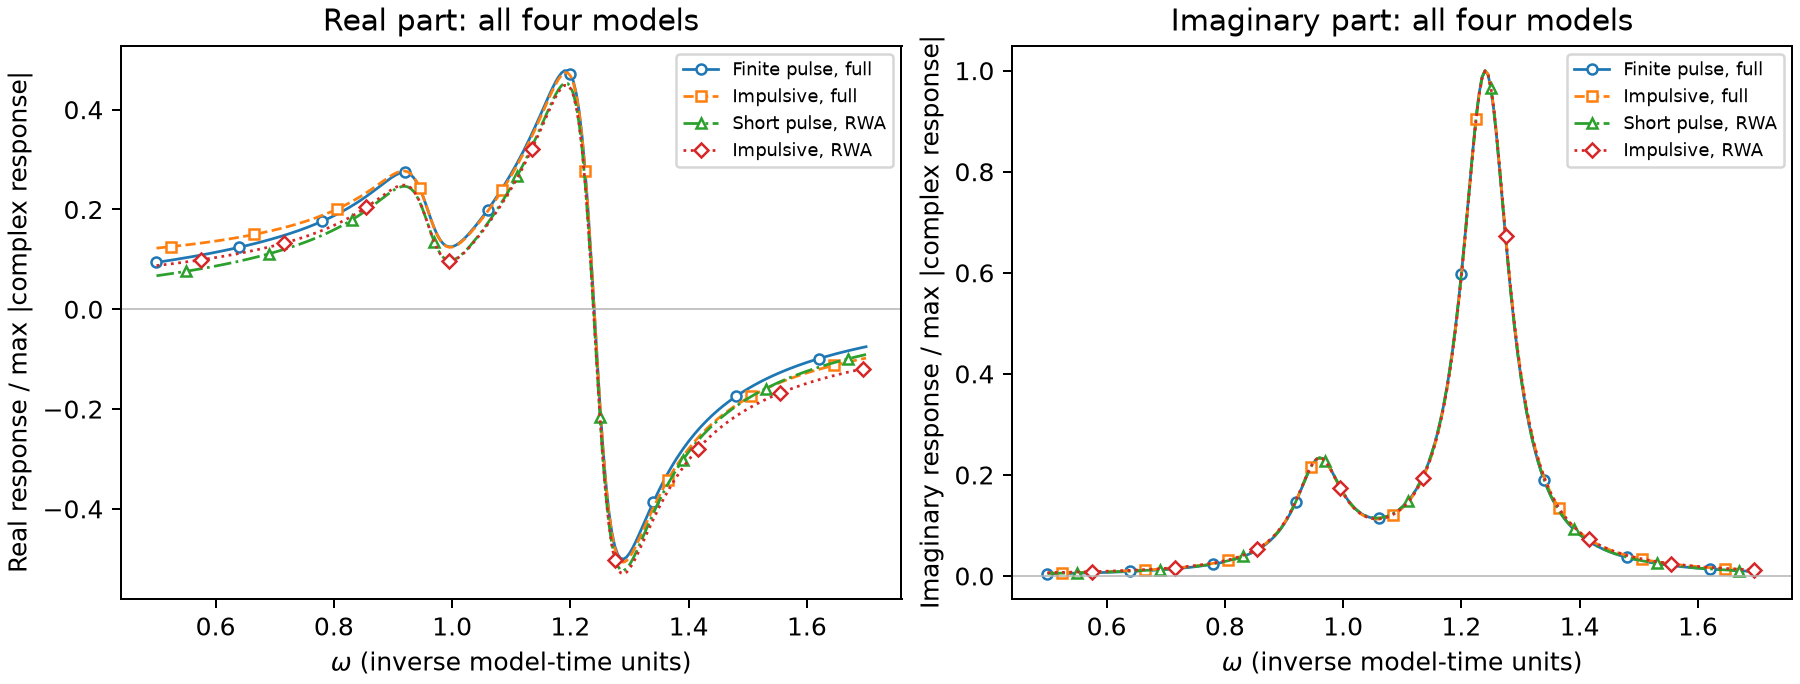
\includegraphics[width=\linewidth]{figures/linear_models.png}
\caption{Real (left) and imaginary (right) parts of the four linear models.
All four curves are present in each panel. For these parameters their
imaginary parts nearly overlap. Distinct line styles are used without markers.
Each complex curve is normalized separately before plotting.}
\label{fig:linear-models}
\end{figure}

\par\noindent
\begin{minipage}{\linewidth}
The script \path{examples/manual/02_linear_models.py} performs this complete
comparison if you have the repository examples. Package-only users can run
the code above after the first example.
\end{minipage}\par

\subsection{Plot and customize a spectrum}

For one curve, the new helper creates a figure when no \texttt{ax} is supplied:
\begin{lstlisting}[style=python]
fig, ax, line = pulsus.plot_linear_spectrum(
    omega, spectra["Finite pulse, full"],
    component="imag", normalize=True,
)
plt.show()
\end{lstlisting}
The default is a line without markers. The helper returns the Matplotlib
figure, axes and line, so labels, colors and other details remain editable.
It neither calls \texttt{plt.show()} nor saves a file by default.
Section~\ref{sec:plot-export} explains optional PNG/PDF export for both
linear and two-dimensional plots.

The calculated spectrum is complex. Use \texttt{S.real}, \texttt{S.imag}, or
\texttt{np.abs(S)} depending on the component you want to inspect. The
functions do not automatically produce a phased absorption coefficient.
Finite-pulse functions include the pulse amplitude and phase; impulsive
functions return the molecular response without these pulse factors.
Record the chosen field scaling when comparing amplitudes across models.

In the finite-pulse full-interaction function, \texttt{sign} selects the
field-frequency component while retaining the complete molecular
interaction. In an RWA function, it also selects the corresponding dipole
interaction. These are distinct choices.

\FloatBarrier
\section{Third-order spectra and approximation models}
\label{sec:third-order}

\subsection{Frequency axes and a common call pattern}

A two-dimensional spectrum is evaluated at fixed waiting time
\texttt{T}. Supply one-dimensional \texttt{omega1} and \texttt{omega3}
axes, not a pair of meshgrid matrices. Every third-order grid function
returns a complex NumPy array with shape
\begin{equation}
 (N_3,N_1)=(\mathrm{len}(\omega_3),\mathrm{len}(\omega_1)).
\end{equation}
Thus \texttt{S[j, i]} is the response at excitation coordinate
\texttt{omega1[i]} and detection coordinate \texttt{omega3[j]}.
The axes need not have equal lengths.

The full finite-pulse signature is
\par\noindent
\begin{minipage}{\linewidth}
\begin{lstlisting}[style=python]
finite_pulse_spectrum(
    system, pulse1, pulse2, pulse3, omega1, omega3, T, eta,
    pathway="NR", rho0=None, signature=None,
)
\end{lstlisting}
\end{minipage}\par
All arguments before \texttt{pathway} are required. The pulses can be
three distinct \texttt{GaussianPulse} objects; reusing one object is only
a convenience in the tutorial. \texttt{T} is the interval used in
$e^{\mathcal L T}$ and must use the same time unit as the pulse widths.
Use nonnegative waiting times. The convergence parameter \texttt{eta}
from Section~\ref{sec:linear} damps the causal transforms for excitation
and detection and broadens their resolvents; it is not inserted into the
waiting-time propagator.
Physical waiting-time decay comes from $\mathcal L$.

\par\noindent
\begin{minipage}{\linewidth}
\begin{lstlisting}[style=python]
omega1 = np.linspace(0.7, 1.5, 31)
omega3 = np.linspace(0.7, 1.5, 31)
S_NR = pulsus.finite_pulse_spectrum(
    system=system,
    pulse1=pulse, pulse2=pulse, pulse3=pulse,
    omega1=omega1, omega3=omega3,
    T=20.0, eta=0.02, pathway="NR", rho0=rho_ss,
)
assert S_NR.shape == (len(omega3), len(omega1))
\end{lstlisting}
\end{minipage}\par
The functions evaluate the frequency-domain formula directly. They do not
first generate a time-domain grid or apply a numerical Fourier transform.

\subsection{Rephasing, nonrephasing, and explicit field signs}

The convenience aliases resolve as
\begin{equation}
 \mathrm{NR}: (+1,-1,+1),\qquad
 \mathrm{R}: (-1,+1,+1).
\end{equation}
Calling \texttt{pulsus.pathway\_signs("NR")} returns the first tuple.
The arguments correspond to signed field-frequency components at the
three ordered interactions. A tuple is a field-sign sector and does not
isolate a single microscopic ground-state-bleaching, stimulated-emission,
or excited-state-absorption diagram.

\texttt{signature=(s1,s2,s3)} accepts any three entries chosen from
$+1$ and $-1$ and overrides \texttt{pathway}. For example,
\par\noindent
\begin{minipage}{\linewidth}
\begin{lstlisting}[style=python]
signs = pulsus.resolve_signature(
    pathway="R", signature=(1, -1, 1),
)
assert signs == (1, -1, 1)  # Explicit tuple takes precedence.
\end{lstlisting}
\end{minipage}\par
Use the alias alone for ordinary R/NR calculations so that a conflicting
tuple cannot accidentally conceal the intended selection.

These aliases do not change the supplied axes. With the repository's
signed-frequency convention, the NR resonances are near positive
$\omega_1$ and positive $\omega_3$, while R resonances are near negative
$\omega_1$ and positive $\omega_3$. Construct the increasing native R axis
explicitly:
\par\noindent
\begin{minipage}{\linewidth}
\begin{lstlisting}[style=python]
omega1_R = -omega1[::-1]
S_R = pulsus.finite_pulse_spectrum(
    system=system,
    pulse1=pulse, pulse2=pulse, pulse3=pulse,
    omega1=omega1_R, omega3=omega3,
    T=20.0, eta=0.02, pathway="R", rho0=rho_ss,
)
\end{lstlisting}
\end{minipage}\par
Passing \texttt{pathway="R"} with an NR positive axis does not reflect
the spectrum automatically. To display R on a positive excitation axis,
reverse its columns together with the axis: use
\texttt{-omega1\_R[::-1]} and \texttt{S\_R[:, ::-1]}.
Axis reflection alone does not implement experimental phasing or turn
R plus NR into a calibrated absorptive measurement.

\subsection{Five available grid models}

There are five third-order grid models. Four form a useful approximation
ladder; a full-interaction impulsive molecular reference is also supplied:
\begin{description}
 \item[A: \texttt{finite\_pulse\_spectrum}]
 Full molecular interaction and operator-valued finite-Gaussian dressing.
 Field signs select pulse components without restricting $\mathcal V$.
 \item[B: \texttt{finite\_pulse\_rwa\_spectrum}]
 The same finite-pulse operator dressing, with each interaction replaced
 by $\mathcal V_+$ or $\mathcal V_-$ according to its field sign.
 \item[C: \texttt{short\_pulse\_rwa\_spectrum}]
 RWA molecular response multiplied by scalar Gaussian spectral
 amplitudes; operator-valued intrapulse dressing is omitted.
 \item[D: \texttt{impulsive\_rwa\_spectrum}]
 RWA molecular response without finite pulse filtering or field
 prefactors.
 \item[Full impulsive reference: \texttt{impulsive\_spectrum}]
 Complete interaction at all three steps, without pulse dressing or
 field prefactors. It has no \texttt{pathway} or \texttt{signature}
 argument.
\end{description}
Models B and C share A's signature. D and the full impulsive reference use
\par\noindent
\begin{minipage}{\linewidth}
\begin{lstlisting}[style=python]
impulsive_rwa_spectrum(
    system, omega1, omega3, T, eta,
    pathway="NR", rho0=None, signature=None,
)
impulsive_spectrum(
    system, omega1, omega3, T, eta, rho0=None,
)
\end{lstlisting}
\end{minipage}\par
The RWA models require both dipole components. The full models need only
the complete dipole. The corresponding \texttt{\_signal} functions have
the same high-level arguments with scalar coordinates and return one
complex number; \texttt{\_response} functions take the matrices and
individual pulse parameters directly. For B, the callable scalar names
\texttt{pulsus.finite\_pulse\_rwa\_signal} and
\texttt{pulsus.finite\_pulse\_rwa\_response} exist even though the
release's \texttt{\_\_all\_\_} list omits those two entries. Prefer
\texttt{import pulsus} and qualified names over wildcard imports.

\subsection{A controlled comparison}

Compare models at identical states, frequency coordinates, waiting time,
and \texttt{eta}. With the RWA-capable tutorial system:
\par\noindent
\begin{minipage}{\linewidth}
\begin{lstlisting}[style=python]
grid = dict(system=system, omega1=omega1, omega3=omega3,
            T=20.0, eta=0.02, rho0=rho_ss)
fields = dict(pulse1=pulse, pulse2=pulse, pulse3=pulse,
              pathway="NR")
A = pulsus.finite_pulse_spectrum(**grid, **fields)
B = pulsus.finite_pulse_rwa_spectrum(**grid, **fields)
C = pulsus.short_pulse_rwa_spectrum(**grid, **fields)
D = pulsus.impulsive_rwa_spectrum(**grid, pathway="NR")
M_full = pulsus.impulsive_spectrum(**grid)
\end{lstlisting}
\end{minipage}\par
The complete example \texttt{examples/manual/03\_third\_order\_models.py}
illustrates A--D for both NR and R. The $A-B$ difference isolates the effect of
the molecular RWA within the same finite-pulse construction. The $B-C$
difference measures replacing operator dressing by scalar field factors
within the RWA. A comparison of $C$ to $D$ must account for the field
prefactors: $D$ is a molecular response rather than the polarization
produced by the specified Gaussian pulses.

More explicitly, the short-pulse expression uses
\[
C(\omega_3,\omega_1)=
E_3^{(s_3)}(\omega_3)E_2^{(s_2)}(-\omega_1)
E_1^{(s_1)}(\omega_1)D(\omega_3,\omega_1).
\]
The minus sign in the second pulse's frequency argument is part of this
convention; do not replace it with $+\omega_1$ when constructing the
expression manually.

For pulse signs $s_k$, define
\begin{equation}
 c_k=\frac{E_{0k}}{2}\sqrt{2\pi}\,\sigma_k e^{is_k\phi_k}.
\end{equation}
A flat-envelope impulsive comparison on the finite-pulse amplitude scale
uses $(c_1c_2c_3)D$. For the equal-pulse NR example,
\par\noindent
\begin{minipage}{\linewidth}
\begin{lstlisting}[style=python]
signs = pulsus.pathway_signs("NR")
area_factor = np.prod([
    pulsus.gaussian_prefactor(
        sigma=pulse.sigma, E0=pulse.E0,
        phase=pulse.phase, sign=s,
    ) for s in signs
])
D_on_field_scale = area_factor * D
\end{lstlisting}
\end{minipage}\par
This restores the signed Gaussian prefactors, not the frequency-dependent
filtering of C. At fixed peak field, reducing all widths to zero also
reduces $c_1c_2c_3$ to zero. A statement about the impulsive limit must
therefore specify fixed peak field, fixed area, or removal of prefactors.

\begin{figure}[!htbp]
\centering
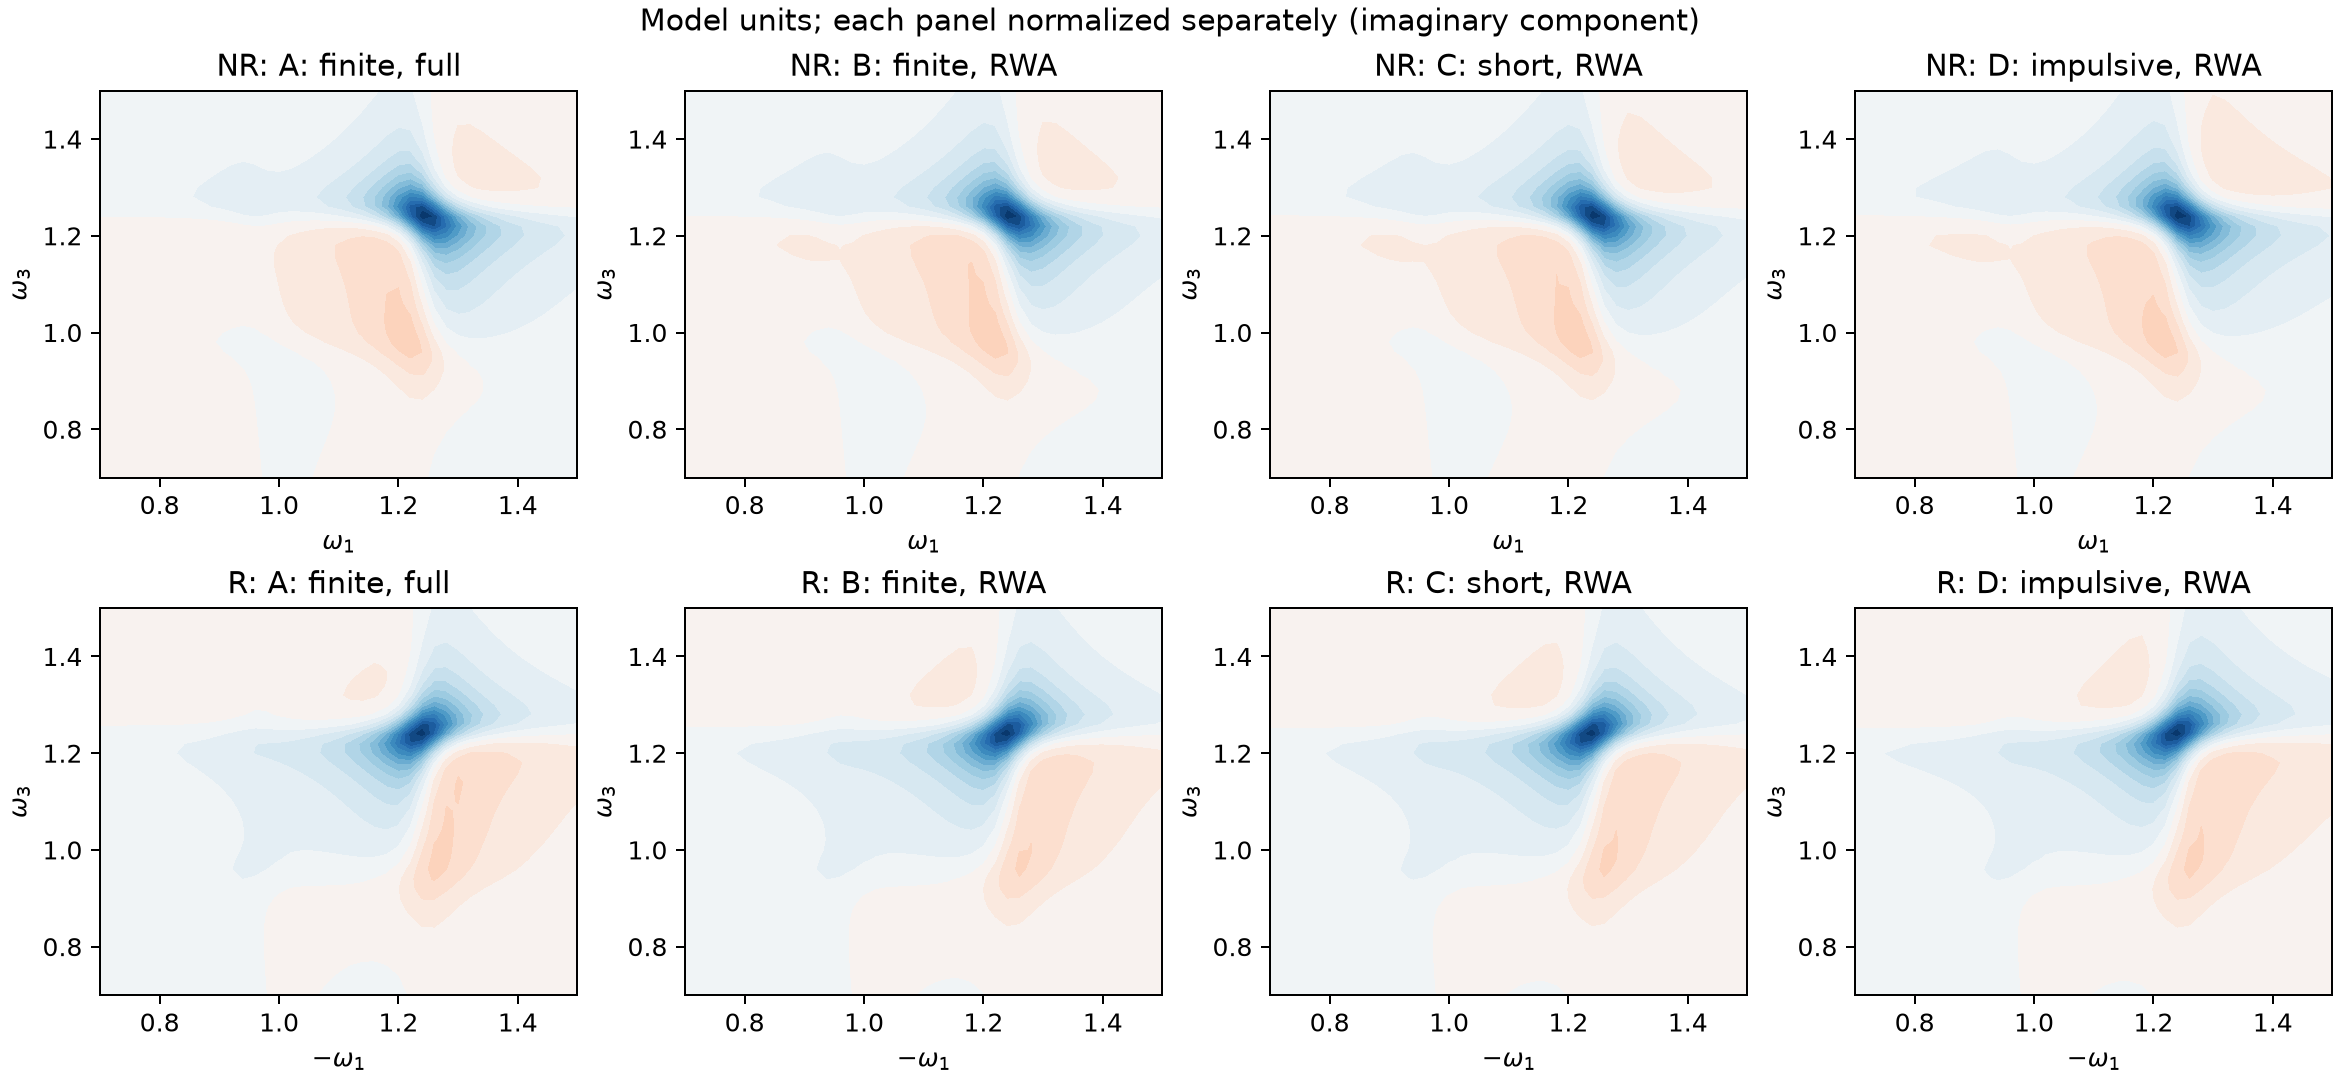
\includegraphics[width=\linewidth]{figures/third_order_models.png}
\caption{A--D for NR (top) and R (bottom), displayed against positive
spectroscopic excitation coordinates. Every panel shows the imaginary
component normalized separately to its maximum absolute value; the
shared red/blue range is $[-1,1]$. This visualization does not preserve
relative amplitudes. The example uses unit Gaussian prefactors at zero pulse phase, $\sigma=1.25$, $T=20$ and $\eta=0.02$.}
\label{fig:third-order-models}
\end{figure}

\subsection{Interpreting plots and convergence}

The array contains a complex response. A contour of its imaginary part
can have positive and negative lobes; its sign is not a population
probability. Interference, field phases, detection convention, and the
selected quadrature all contribute. A single colored lobe should not be
assigned to one microscopic diagram solely from this plot.

Normalized contour plots help inspect shape, but retain the original
complex arrays for amplitude comparisons. Refine axes until the features
used in the analysis are stable; grid agreement does not remove
approximation error. Vary pulse width and \texttt{eta} independently,
and distinguish physical broadening in $\mathcal L$ from convergence
broadening. The finite-pulse APIs implement the repository's ordered
Gaussian dressing model; the word ``finite'' does not turn this into a
general numerical propagation of an arbitrary overlapping pulse train.

\FloatBarrier
\section{Selected coordinates and time-domain calculations}
\label{sec:coordinates}

\subsection{Compute pairs without building a Cartesian grid}

Use \texttt{finite\_pulse\_points} when only a diagonal cut, a few peak
coordinates, or a prescribed path through frequency space is needed. Its
signature matches \texttt{finite\_pulse\_spectrum}:
\par\noindent
\begin{minipage}{\linewidth}
\begin{lstlisting}[style=python]
finite_pulse_points(
    system, pulse1, pulse2, pulse3, omega1, omega3, T, eta,
    pathway="NR", rho0=None, signature=None,
)
\end{lstlisting}
\end{minipage}\par
Here the two frequency arrays must be one-dimensional and have equal
length. Entry $k$ requests the pair
$(\omega_1[k],\omega_3[k])$. The result has shape \texttt{(N,)} rather
than \texttt{(N, N)}. Repeated excitation and detection values are cached
internally. This API computes the full finite-pulse model; there is no
dedicated RWA selected-points wrapper in 0.2.0.

\par\noindent
\begin{minipage}{\linewidth}
\begin{lstlisting}[style=python]
cut = np.linspace(0.7, 1.5, 61)
diagonal = pulsus.finite_pulse_points(
    system=system,
    pulse1=pulse, pulse2=pulse, pulse3=pulse,
    omega1=cut, omega3=cut,
    T=20.0, eta=0.02, pathway="NR", rho0=rho_ss,
)
assert diagonal.shape == (len(cut),)
\end{lstlisting}
\end{minipage}\par
This evaluates the diagonal directly without calculating all
$61^2$ combinations. For an R diagonal in native coordinates, supply
\texttt{omega1=-cut} and \texttt{omega3=cut} with
\texttt{pathway="R"}. The pairs retain their supplied order.

When comparing points with an existing grid, preserve its row/column
ordering:
\par\noindent
\begin{minipage}{\linewidth}
\begin{lstlisting}[style=python]
rows = np.array([0, 10, 20])  # omega3 indices
cols = np.array([5, 15, 25])  # omega1 indices
values = pulsus.finite_pulse_points(
    system=system,
    pulse1=pulse, pulse2=pulse, pulse3=pulse,
    omega1=omega1[cols], omega3=omega3[rows],
    T=20.0, eta=0.02, pathway="NR", rho0=rho_ss,
)
assert np.allclose(values, S_NR[rows, cols])
\end{lstlisting}
\end{minipage}\par
The two integer arrays above select three paired entries, not a
three-by-three subgrid. The complete example is
\texttt{examples/manual/04\_selected\_points.py}.

\begin{figure}[!htbp]
\centering
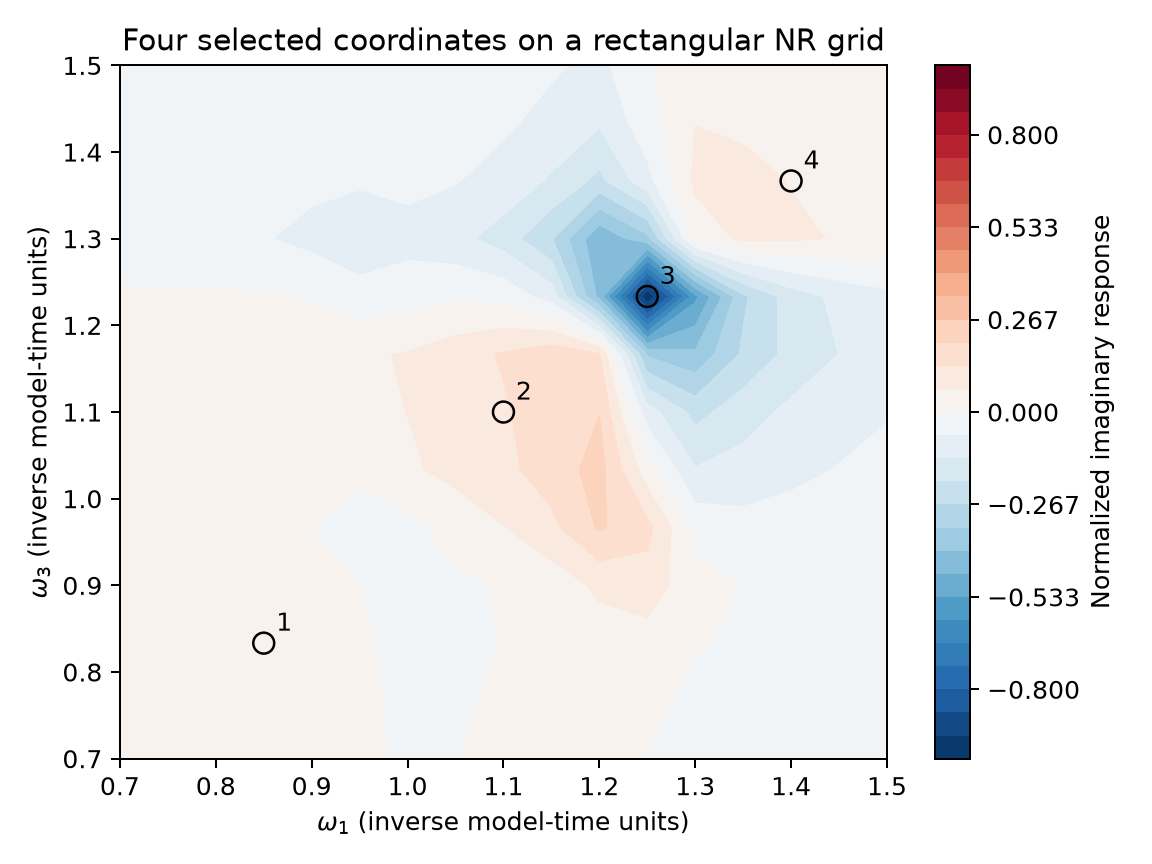
\includegraphics[width=0.75\linewidth]{figures/selected_points.png}
\caption{Four paired coordinates on a $13\times17$ Cartesian grid.
The numbered circles mark the pairs evaluated by
\texttt{finite\_pulse\_points}; their complex values agree with the
corresponding grid entries. The background is a normalized imaginary
NR response, sampled coarsely for this indexing demonstration.}
\label{fig:selected-points}
\end{figure}

\subsection{A generic grid evaluator}

\texttt{response\_grid(response\_function, omega1, omega3, **kwargs)}
calls a scalar response function for every Cartesian pair. The function
must accept \texttt{omega1} and \texttt{omega3} as keyword arguments.
For example,
\par\noindent
\begin{minipage}{\linewidth}
\begin{lstlisting}[style=python]
S_check = pulsus.response_grid(
    pulsus.impulsive_rwa_signal,
    omega1=omega1, omega3=omega3,
    system=system, T=20.0, eta=0.02,
    pathway="NR", rho0=rho_ss,
)
\end{lstlisting}
\end{minipage}\par
The return shape is again $(N_3,N_1)$. Prefer the dedicated spectrum
wrappers for routine calculations: their caching avoids rebuilding
frequency-dependent objects at every pair. The generic evaluator is useful
for an explicitly defined scalar response or a small independent check.
To obtain a few RWA coordinates, call its scalar \texttt{\_signal}
function in a loop rather than constructing a full Cartesian grid.

\subsection{Delay-domain response functions}
\label{sec:time-domain}

The public time-domain API uses impulsive interactions. It evaluates
matrix-exponential propagation, and these functions have no
\texttt{GaussianPulse} or \texttt{eta} argument. Nonnegative,
one-dimensional time axes are required. Four functions return response
arrays on delay axes:
\par\noindent
\begin{minipage}{\linewidth}
\begin{lstlisting}[style=python]
impulsive_linear_time_signal(system, times, rho0=None)
impulsive_linear_rwa_time_signal(
    system, times, sign=1, rho0=None)
impulsive_third_order_time_signal(
    system, t1, t3, T, rho0=None)
impulsive_third_order_rwa_time_signal(
    system, t1, t3, T,
    pathway="NR", signature=None, rho0=None)
\end{lstlisting}
\end{minipage}\par
The linear results have shape \texttt{(len(times),)}. The third-order
results have shape \texttt{(len(t3), len(t1))}, with nonnegative
\texttt{T}. All are complex NumPy arrays. The full-interaction third-order
response is
\begin{equation}
 R^{(3)}(t_3,T,t_1)=\langle\!\langle\mu|
 e^{\mathcal L t_3}\mathcal V e^{\mathcal L T}
 \mathcal V e^{\mathcal L t_1}\mathcal V
 |\rho_0\rangle\!\rangle.
\end{equation}
The RWA version replaces the three interactions according to the resolved
field signs and requires both dipole components.

\par\noindent
\begin{minipage}{\linewidth}
\begin{lstlisting}[style=python]
times = np.linspace(0.0, 60.0, 301)
R1 = pulsus.impulsive_linear_time_signal(
    system=system, times=times, rho0=rho_ss,
)
t1 = np.linspace(0.0, 20.0, 41)
t3 = np.linspace(0.0, 20.0, 41)
R3 = pulsus.impulsive_third_order_rwa_time_signal(
    system=system, t1=t1, t3=t3, T=20.0,
    pathway="NR", rho0=rho_ss,
)
\end{lstlisting}
\end{minipage}\par
Time axes are sampled at the values supplied; uniform spacing is not
required by the propagator API. A numerical FFT would impose additional
sampling and transform conventions that these functions do not supply.

\subsection{Laboratory-time polarization traces}

Two functions place the impulsive response on an absolute time axis:
\par\noindent
\begin{minipage}{\linewidth}
\begin{lstlisting}[style=python]
impulsive_linear_polarization(
    system, times, pulse_time=0.0, sign=None, rho0=None)
impulsive_third_order_polarization(
    system, times, pulse_times,
    pathway=None, signature=None, rho0=None)
\end{lstlisting}
\end{minipage}\par
Both return a complex vector of length \texttt{len(times)}. In the linear
function, \texttt{sign=None} uses the full interaction; $+1$ or $-1$ uses
its RWA component. The response is zero before the nonnegative
\texttt{pulse\_time} and is evaluated at delay
\texttt{times - pulse\_time} afterwards.

In the third-order function, \texttt{pulse\_times} must contain exactly
$(\tau_1,\tau_2,\tau_3)$ with
$0\leq\tau_1\leq\tau_2\leq\tau_3$. It sets
$t_1=\tau_2-\tau_1$ and $T=\tau_3-\tau_2$, and returns zero before
$\tau_3$. If both \texttt{pathway} and \texttt{signature} are
\texttt{None}, all three interactions are full. Supplying either
selects the RWA field-sign sector, with an explicit signature taking
precedence.

\par\noindent
\begin{minipage}{\linewidth}
\begin{lstlisting}[style=python]
lab_times = np.linspace(0.0, 70.0, 351)
P3 = pulsus.impulsive_third_order_polarization(
    system=system, times=lab_times,
    pulse_times=(5.0, 10.0, 30.0),
    pathway="NR", rho0=rho_ss,
)
assert np.allclose(P3[lab_times < 30.0], 0.0)
\end{lstlisting}
\end{minipage}\par
The initial state in these functions is used directly at the first
interaction. The implementation does not propagate it from laboratory
time zero to $\tau_1$ or \texttt{pulse\_time}. A stationary state is
unchanged by that omitted free interval. For a nonstationary preparation,
propagate or otherwise specify the state just before the first pulse.
These traces do not include independently specified pulse amplitudes.

\subsection{Piecewise pathway history is a different object}

The seventh public time-domain function is
\par\noindent
\begin{minipage}{\linewidth}
\begin{lstlisting}[style=python]
impulsive_pathway_polarization(
    system, times, pulse_times, pathway="NR",
    signature=None, rho0=None, return_components=False)
\end{lstlisting}
\end{minipage}\par
It always uses RWA interactions and shows successive stages of one
ordered field-sign history: first-order coherence between pulses 1 and 2,
the second-order state between pulses 2 and 3, and third-order
polarization from pulse 3 onward. The projection onto the dipole can
vanish during a stage even though the intermediate density operator is
nonzero.

With \texttt{return\_components=True}, the return value is a tuple:
\par\noindent
\begin{minipage}{\linewidth}
\begin{lstlisting}[style=python]
history, components = pulsus.impulsive_pathway_polarization(
    system=system, times=lab_times,
    pulse_times=(5.0, 10.0, 30.0),
    pathway="NR", rho0=rho_ss, return_components=True,
)
P1_stage = components["first_order"]
P2_stage = components["second_order"]
P3_stage = components["third_order"]
assert np.allclose(history, P1_stage + P2_stage + P3_stage)
\end{lstlisting}
\end{minipage}\par
The three arrays have disjoint stage masks. Earlier orders are set to
zero after their displayed stage. Thus \texttt{history} is a piecewise
diagnostic visualization, not the total physical polarization including
all simultaneously present orders and all pulse interactions. Use
\texttt{impulsive\_third\_order\_polarization} when the desired quantity
is strictly the third-order contribution after the third pulse.
The complete tutorial script
\path{examples/manual/05_time_domain.py} illustrates both objects.

\begin{figure}[!htbp]
\centering
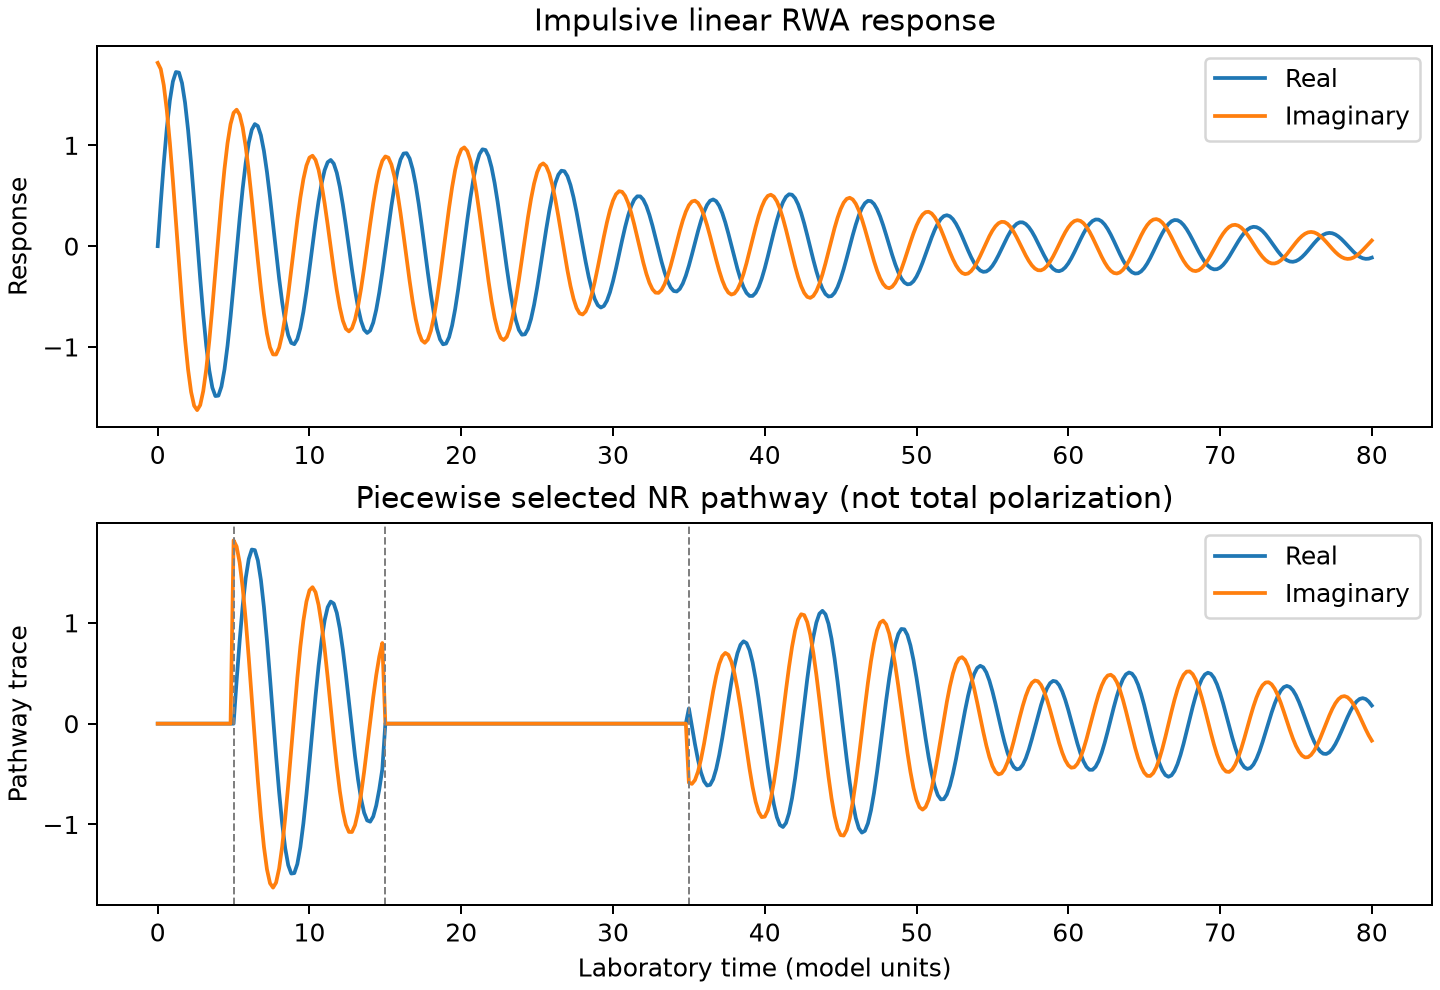
\includegraphics[width=0.9\linewidth]{figures/time_domain.png}
\caption{Impulsive linear RWA response (top) and the selected NR
pathway's piecewise history (bottom). Dashed lines mark pulses at model
times 5, 15 and 35. The stage trace after the third pulse agrees with the
strict third-order polarization for the same ordered sequence. Earlier
orders are not retained after their displayed stage.}
\label{fig:time-domain}
\end{figure}


\FloatBarrier
\section{Practical checks}
\label{sec:validation}

Before increasing the size of a calculation, check these four choices:
\begin{description}
\item[Units.] Use one time unit throughout. Frequencies, decay rates and
\texttt{eta} are in its inverse; pulse widths and delays are in that unit.
With physical Hamiltonian energies, use the matching value of $\hbar$.
\item[Initial state.] Pass the intended density matrix explicitly.
For stationary preparation, use \texttt{rho0=rho\_ss} after computing
\texttt{rho\_ss = system.stationary\_state()}.
\item[Frequency grid.] Start with a small grid, then reduce the spacing
around peaks until their shape and amplitude stop changing appreciably.
The result is indexed as \texttt{S[omega3\_index, omega1\_index]}.
\item[Convergence parameter.] Use a small positive \texttt{eta} to ensure
causal-transform convergence. Reduce it while refining the frequency grid
until its added broadening no longer materially changes the features of
interest and the linear solves remain stable. Check unnormalized complex
responses so normalization does not hide amplitude changes.
\end{description}

Detailed checks of the implementation and time--frequency comparisons
are kept separately in \path{docs/VALIDATION.md} and
\path{docs/advanced_notes.md}.

\FloatBarrier
\section{Troubleshooting and practical recipes}
\label{sec:troubleshooting}

\subsection{Installation and environment}
\begin{description}[style=nextline]
\item[\texttt{ModuleNotFoundError: No module named 'pulsus'}]
Activate the intended environment and install with
\texttt{python -m pip install pulsus-spec}. Print
\texttt{sys.executable} and \texttt{pulsus.\_\_file\_\_} to identify the
interpreter and source actually used. Avoid naming your own script
\texttt{pulsus.py}, which can shadow the package.
\item[Notebook imports a different version.]
Select the kernel belonging to the spectroscopy environment. If needed,
install \texttt{ipykernel} in that environment and register it:
\par\noindent
\begin{minipage}{\linewidth}
\begin{lstlisting}[style=shell]
python -m pip install ipykernel
python -m ipykernel install --user --name pulsus --display-name "Python (PULSUS)"
\end{lstlisting}
\end{minipage}\par
Restart the selected kernel after updating a package already imported there.
\item[An example cannot import \texttt{dimer\_model} or \texttt{common}.]
The older development examples may use \texttt{src/dimer\_model.py}, which is
not an installed public PULSUS module. This manual's first example is
self-contained. Run examples~02--05 as scripts from the checkout, keeping
their \texttt{common.py} helper beside them; do not copy those scripts alone
and expect the helper to come from PyPI.
\end{description}

\subsection{States and operators}
\begin{description}[style=nextline]
\item[\texttt{An initial state must be supplied ...}]
Computing \texttt{rho\_ss = system.stationary\_state()} does not populate
\texttt{system.rho0}. Pass \texttt{rho0=rho\_ss} to the calculation, or assign
a suitable initial state when constructing the system. A call-level
\texttt{rho0} overrides the stored state.
\item[\texttt{RWA calculations require dipole\_plus and dipole\_minus ...}]
Supply both matrices to \texttt{SpectroscopySystem}. Check
$\mu=\mu_++\mu_-$ and, for a Hermitian dipole, $\mu_-=\mu_+^\dagger$.
The package does not infer the decomposition from $H$ automatically.
\item[Stationary state is ambiguous or appears unphysical.]
The eigenvector-based routine chooses the eigenvalue closest to zero. A
generator with multiple stationary states does not specify a unique
preparation. Check trace, Hermiticity, eigenvalues and residual, then supply
the state that represents the experiment. Adding arbitrary relaxation solely
to force uniqueness changes the physical model.
\item[Relaxation is much faster or slower than expected.]
Collapse operators contain the square root of a rate. Using $\gamma A$
where $\sqrt{\gamma}A$ was intended changes the dissipative rate to a quantity
proportional to $\gamma^2$. Also check that $H/\hbar$, rates, angular
frequencies and time parameters use compatible units.
\end{description}

\Needspace{12\baselineskip}
\subsection{Coordinates, amplitudes and plotting}
\begin{description}[style=nextline]
\item[The rephasing signal is absent on a positive excitation axis.]
The calculation uses negative \texttt{omega1} for the standard R sector.
\texttt{pathway="R"} selects interaction signs but does not flip coordinates.
Calculate on the negative axis, then display against $-\omega_1$ if desired.
\item[A spectrum appears transposed.]
Grid outputs have shape $(N_3,N_1)$, with detection on rows. Use unequal
axis lengths to diagnose orientation. Pair coordinates with
\texttt{finite\_pulse\_points}; do not reshape its $(N,)$ output into a
Cartesian grid unless you explicitly constructed and ordered that grid.
\item[Changing \texttt{pathway} has no effect.]
Check whether an explicit \texttt{signature} is also supplied. That tuple
overrides the pathway alias. Also distinguish full impulsive functions,
which do not have a pathway argument, from sector-selecting RWA functions.
\item[The plotted sign or amplitude is surprising.]
The response is complex. Choose \texttt{real}, \texttt{imag} or \texttt{abs}
deliberately and record the phase and normalization conventions. The plotter
defaults to the real component without normalization. Negative signed
components are valid. Normalizing each plot separately removes absolute
amplitude information and is unsuitable for amplitude-error comparisons.
\item[Very narrow pulses give a small signal.]
At fixed peak field, each Gaussian signed-component area scales as
$E_0\sigma$. Narrowing the pulse therefore also reduces its area. If the
purpose is an impulsive-limit comparison at fixed area, adjust $E_0$
consistently rather than comparing unlike field strengths.
\item[Values are nonfinite or unexpectedly large.]
Check input units, pulse widths, physical rates and stationarity first.
The Gaussian dressing contains matrix exponentials; extreme parameter
choices can expose numerical conditioning or fall outside the separated-pulse
regime. Start from the validated small example and change one parameter at a
time. Do not hide nonfinite values by normalizing or clipping the plot.
\end{description}

\subsection{Prepare a custom model}
Begin with a small truncated Hamiltonian, a dipole in the same basis and
physically justified collapse operators. Verify state preparation and a
linear spectrum before building a large third-order grid. For an electronic
or vibronic RWA calculation, define the raising/lowering decomposition in
the intended excitation manifolds. Then compare approximations on identical
coordinates using a documented pulse-amplitude convention.

\clearpage
\section{Function guide}
\label{sec:api-reference}

The functions below cover most everyday calculations. API means
\emph{application programming interface}: the public classes and
functions you call from Python. The complete reference, including
less frequently used utilities and every exact signature, is in
\path{docs/api.md}.

\subsection{The functions you will use most}

\begin{tabular}{@{}p{0.39\linewidth}p{0.56\linewidth}@{}}
\toprule
\textbf{Function or class} & \textbf{When to use it} \\
\midrule
\texttt{SpectroscopySystem} & Define the Hamiltonian, dipole, dissipation
and optional initial state. \\
\texttt{GaussianPulse} & Set a Gaussian pulse's carrier frequency, temporal
width, amplitude and phase. \\
\texttt{system.stationary\_state()} & Obtain a stationary initial density
matrix; pass it as \texttt{rho0} in the calculation. \\
\texttt{*\_spectrum} & Calculate the frequency array you will normally
plot: a 1D linear spectrum or a 2D third-order spectrum. \\
\texttt{plot\_linear\_spectrum} & Plot one component of a 1D linear spectrum;
pass an existing axis to overlay curves. \\
\texttt{plot\_spectrum} & Plot one component of a 2D spectrum on its
Cartesian frequency grid. \\
\texttt{finite\_pulse\_points} & Calculate selected frequency pairs
without building a full 2D grid. \\
\bottomrule
\end{tabular}

\subsection{What do signal, spectrum, and response mean?}

Choose a model prefix, such as \texttt{finite\_pulse} or
\texttt{impulsive\_rwa}; its suffix tells you how to supply inputs
and what is returned:
\begin{description}
\item[\texttt{\_spectrum}.] Use a system object and frequency arrays.
The result is a complex array: \texttt{(N,)} for linear spectroscopy,
or \texttt{(N3, N1)} for third order.
\item[\texttt{\_signal}.] Use a system object and a single frequency
coordinate. The result is one complex number. Use this for one peak or
one selected pair rather than a complete plot.
\item[\texttt{\_response}.] Supply the Liouvillian, interaction and
detection matrices directly. The result is one complex number.
These functions are useful when working directly with superoperators;
most users can use \texttt{\_signal} or \texttt{\_spectrum} instead.
\item[\texttt{\_time\_signal}.] Supply delay-time arrays instead of
frequencies. The result is a complex time-domain array. All such functions
in this version use impulsive interactions.
\end{description}

These are interface names: \texttt{signal} does not add a detector model.
For example, the finite-pulse NR response can be evaluated at one pair
or across a full Cartesian grid:
\par\noindent
\begin{minipage}{\linewidth}
\begin{lstlisting}[style=python]
value = pulsus.finite_pulse_signal(
    system, pulse, pulse, pulse, 1.24, 1.24,
    T=20.0, eta=0.02, pathway="NR", rho0=rho_ss,
)  # one complex number
S = pulsus.finite_pulse_spectrum(
    system, pulse, pulse, pulse, omega1, omega3,
    T=20.0, eta=0.02, pathway="NR", rho0=rho_ss,
)  # shape (len(omega3), len(omega1))
\end{lstlisting}
\end{minipage}\par

\clearpage
\subsection{Common calling patterns}

The three third-order Gaussian-pulse models use the same arguments:
\par\noindent
\begin{minipage}{\linewidth}
\begin{lstlisting}[style=python]
finite_pulse_spectrum(
    system, pulse1, pulse2, pulse3, omega1, omega3, T, eta,
    pathway="NR", rho0=None, signature=None)
finite_pulse_rwa_spectrum(
    system, pulse1, pulse2, pulse3, omega1, omega3, T, eta,
    pathway="NR", rho0=None, signature=None)
short_pulse_rwa_spectrum(
    system, pulse1, pulse2, pulse3, omega1, omega3, T, eta,
    pathway="NR", rho0=None, signature=None)
\end{lstlisting}
\end{minipage}\par
The impulsive models take no pulse object:
\par\noindent
\begin{minipage}{\linewidth}
\begin{lstlisting}[style=python]
impulsive_spectrum(
    system, omega1, omega3, T, eta, rho0=None)
impulsive_rwa_spectrum(
    system, omega1, omega3, T, eta,
    pathway="NR", rho0=None, signature=None)
\end{lstlisting}
\end{minipage}\par
Replacing \texttt{\_spectrum} with \texttt{\_signal} in any of these
five names keeps the arguments but requires scalar frequencies.
\texttt{finite\_pulse\_points} uses the finite-pulse signature with
paired arrays of equal length and returns an \texttt{(N,)} array.

For linear spectroscopy, the four spectrum functions are
\par\noindent
\begin{minipage}{\linewidth}
\begin{lstlisting}[style=python]
finite_pulse_linear_spectrum(
    system, pulse, omega, eta, sign=1, rho0=None)
short_pulse_linear_rwa_spectrum(
    system, pulse, omega, eta, sign=1, rho0=None)
impulsive_linear_spectrum(system, omega, eta, rho0=None)
impulsive_linear_rwa_spectrum(
    system, omega, eta, sign=1, rho0=None)
\end{lstlisting}
\end{minipage}\par
Here \texttt{omega} is one 1D axis. Replacing \texttt{\_spectrum} with
\texttt{\_signal} takes one frequency and returns one complex number.
There is no separate finite-pulse linear RWA family in this version.

\subsection{Plot, customize and optionally save}
\label{sec:plot-export}

Both plotting helpers return Matplotlib objects. They create a figure if
\texttt{ax} is omitted, and draw on that axis if it is supplied:
\par\noindent
\begin{minipage}{\linewidth}
\begin{lstlisting}[style=python]
linear_spectrum = spectra["Finite pulse, full"]
fig, ax, line = pulsus.plot_linear_spectrum(
    omega, linear_spectrum, component="imag", normalize=True,
)
plt.show()

fig, ax, contour = pulsus.plot_spectrum(
    omega1, omega3, S, component="imag", normalize=True,
)
plt.show()
\end{lstlisting}
\end{minipage}\par
Use \texttt{component="real"}, \texttt{"imag"}, or \texttt{"abs"}.
Normalization scales only the displayed component; it does not modify
the complex input array. The linear helper accepts ordinary line options,
such as \texttt{linestyle="--"}, \texttt{color="navy"} and a curve
\texttt{label}; add \texttt{ax.legend()} when comparing labeled curves.
Neither helper displays or saves automatically. Use \texttt{plt.show()}
when running a script.

Both helpers accept \texttt{savepath=None} and \texttt{dpi=300}.
Omitting \texttt{savepath} writes nothing. Supply a filename to export the
figure immediately; its extension selects the format:
\begin{lstlisting}[style=python]
fig, ax, line = pulsus.plot_linear_spectrum(
    omega, linear_spectrum, component="imag",
    savepath="linear_spectrum.png", dpi=300,
)
# Use savepath="linear_spectrum.pdf" for PDF output.
\end{lstlisting}
The same two optional arguments work with \texttt{plot\_spectrum}.
Use an existing destination folder. The resolution controls raster
output; PDF line work remains vector graphics.

For additional curves, legends or other customization, omit
\texttt{savepath} and export the completed figure afterward:
\begin{lstlisting}[style=python]
ax.set_title("My spectrum")
fig.savefig("custom_spectrum.pdf", dpi=300, bbox_inches="tight")
plt.show()
\end{lstlisting}
Saving a figure exports its visual appearance, not the complex numerical
spectrum. The input array remains available for analysis and separate data
storage.

Refer to Section~\ref{sec:time-domain} for time-domain
functions and to \path{docs/api.md} for lower-level response functions,
Liouville-space utilities, resolvents, and Gaussian dressing functions.

\end{document}
